\documentclass[fleqn,10pt]{physiome}

% Further packages
\usepackage{siunitx}
\usepackage{placeins}

\articletype{Retrospective}
%% Choose from Original, Retrospective, Review, Letter

\title{Spindle Model Responsive to Mixed Fusimotor Inputs: an updated version of the Maltenfort and Burke (2003) model}

\author[1][laura.schmid@imsb.uni-stuttgart.de]{Laura Schmid}
\author[1]{Thomas Klotz}
\author[2]{Utku {\c S}. Yavuz}
\author[3]{Mitchell Maltenfort}
\author[1,4]{Oliver R{\"o}hrle}
\affil[1]{Institute for Modelling and Simulation of Biomechanical Systems, University of Stuttgart, Germany}
\affil[2]{Department of Biomedical Signals and Systems, Faculty of Electrical Engineering, Mathematics and Computer Sciences, University of Twente, Netherlands}
\affil[3]{The Applied Clinical Research Center, Department of Biomedical and Health Informatics, Children's Hospital of Philadelphia, USA}
\affil[4]{Stuttgart Center for Simulation Sciences (SC SimTech), University of Stuttgart, Germany}

%% The following lines can be omitted when submitting;
%% information will be added by editors
\publicationdate{27 Jan 2022}
\editor{Shelley Fong}
\curator{Karin Lundengård}
\submitteddate{12 Jan 2022}
\accepteddate{20 Jan 2022}
\citethisas{Schmid et al. (2022)\\Spindle Model Responsive to Mixed Fusimotor Inputs: an updated version of the Maltenfort and Burke (2003) model. Physiome.}{10.36903/physiome.19070171}
\begin{document}

\maketitle

\begin{abstract}
%Please provide an abstract of no more than 300 words. Your abstract should explain the main contributions of your article, and should not contain any material that is not included in the main text. \\
The muscle spindle model presented in \citet{maltenfort2003} calculates muscle spindle primary afferent feedback depending on the muscle fibre stretch and fusimotor drive. 
The aim of this paper is to provide an updated version of the model, which is now capable of replicating the originally published data. 
This is achieved by modifying the equations describing the modulation of the muscle spindle output in response to dynamic fusimotor drive. 
\end{abstract}

\keywords{muscle spindle, afferent feedback, proprioception, neuromuscular system}

% To DO: Provide link to model in []
\primarypubs[10.36903/physiome.19070171]{MB03}{maltenfort2003}

\section{Introduction}
% Brief explanation of the biological system modelled. Reference data used for validation and previously published versions of the model. 
Muscle spindles can be found in almost all skeletal muscles and make the most important contribution to proprioception~\citep{macefield2018}. The muscle spindle is a special mechano-receptor sensing the intrafusal muscle fiber length change and providing stretch feedback to the neuromuscular system via two types of axons: primary~(Ia) and secondary~(II) fibers.
The afferent axons form feedback loops exciting $\alpha$-motoneurons and thus, ultimately control skeletal muscle contraction \citep{kandel2000}. 
For optimizing motor control in various conditions, the sensitivity of muscle spindles is modulated by specialized neurons, i.\,e. skeletofusimotor ($\beta$)- as well as static and dynamic fusimotor ($\gamma$)-neurons \citep{banks1994,matthews1962}. \\
The muscle spindle model by \citet{maltenfort2003} predicts primary afferent feedback depending on the muscle stretch and fusimotor drive. The model was validated using data recorded from cat muscle spindles during ramp-and-hold and sinusoidal stretches \citep{crowe1964,hulliger1977a,hulliger1977b}. 
%The model matches the experimental data in the range of experimental variability. 
The strength of the model is its capability to predict muscle spindle primary activity over a large range of physiological conditions while demanding little computational resources.\\
However, in the presence of dynamic fusimotor drive, the published model predicts spindle frequencies that are considerably higher than shown in the original publication.  
\citet{grandjean2014} previously adapted the \citet{maltenfort2003} model to improve the predicted physiological behaviour in the presence of fusimotor drive. However, they did not publish their code and the shown results could not be reproduced with the provided equations.
Thus, the aim of this manuscript is to provide an updated and validated version of the muscle spindle model originally published in \citet{maltenfort2003}.
In detail, this work presents a model capable of replicating the muscle spindle firing rates during ramp-and-hold and sinusoidal stretches while considering variable fusimotor drives as shown in Fig.~4 and Fig.~5 of the original publication. 
Since the published equations are based on a specific discretization scheme and hence, the time step size is a variable, the model is implemented in MATLAB. 
Nevertheless, to promote the use of open standards for model sharing, we additionally provide a CellML implementation of the updated model. \\
Note that we will refer to the model based on the equations published in \citet{maltenfort2003} as original model and to our model as the updated model. 

% Modifications by Grandjean: 
% - Add acceleration dependent component
% - Replaced occlusion function by a fixed coefficiant of interaction
% - Adapted functions Svd, Qd (both with typos in Maltenfort paper and corrected here) and Svs to better fit experimental data under fusimotor drive
% - They modified the equations from the paper, not the corrected ones!

% Maltenfort and Burke beta drive: implemented like a new gamma drive. No new equations needed. 


\section{Model description}
% An overview of the type of model and its structure.
The Maltenfort and Burke muscle spindle model was developed for two purposes: the investigation  of $\beta$-feedback loops~\citep{burke1977} and for serving as computationally efficient model in large-scale simulations of the neuromuscular system.  
The latter is ensured by employing only algebraic equations. 
The model has a block-wise structure (cf. Fig.~1B in the original manuscript), calculating a baseline muscle spindle frequency for passive length changes as well as additional contributions modulated by static and dynamic fusimotor drives. Following the findings from \citet{andersson1968}, \citet{lennerstrand1968b,lennerstrand1968c} and \citet{lennerstrand1968a} and using a phenomenological approach, each contribution is calculated as the sum of four components: a pure velocity and a pure position sensitivity, a mixed velocity and position sensitivity and a baseline firing rate at the initial length.
Thereby, the velocity is the filtered derivative of the the position input to achieve smooth transitions from shortening to lengthening (cf. \citet{maltenfort2003}, Eqn. 3).  
The static and dynamic contributions are non-linearly mixed by an occlusion function, partially suppressing the smaller contribution as it was observed in experimental studies \citep{schafer1974}.
Finally, the passive contribution and the mixed fusimotor contribution are added up yielding the firing rate of the muscle spindle primary axon. \\
Since the role of $\beta$-innervation is still under debate, the $\beta$-feedback loop is not part of the provided model.  

\section{Model modifications}\label{sec:modifications}
% Any modifications made to the model, including motivations and origin. 
Comparisons with the original code, which was kindly provided by the author, revealed deviations with respect to the published equations. This exclusively concerns the descriptions of the velocity-dependent terms modulated by dynamic fusimotor drive $Q_{\mathrm d}$ and $S_\mathrm{v,d}$ from Table~1 in the original manuscript. For better comprehensibility of the quantities and their context, we will display further equations. 
The parameter values are all adopted from the original publication.\\
Note that the modifications introduced in Section \ref{sec:mod_matlab} apply to both provided implementations, i.\,e. MATLAB and CellML, while the modifications introduced in Section \ref{sec:mod_cellml} only apply to the CellML implementation. 
%
\subsection{General model modifications}\label{sec:mod_matlab}
Eqn.~2A of the original paper models the muscle spindle Ia firing rate $R$ as the sum of a passive contribution $R_{\mathrm{passive}}$ and the mixed contribution from static ($\Delta R_{\mathrm{static}}$) and dynamic ($\Delta R_{\mathrm{dynamic}}$) fusimotor drive:
%
\begin{equation}
    R \ = \ R_{\mathrm{passive}} \ + \ f_{\mathrm{occlusion}}\left( \Delta R_{\mathrm{dynamic}},\Delta R_{\mathrm{static}} \right)
\end{equation}
%
Thereby, $f_{\mathrm{occlusion}}$ is a function describing the non-linear summation of the contributions from static and dynamic fusimotor input. \\
In detail, the contribution modulated by dynamic fusimotor drive $\Delta R_{\mathrm{dynamic}}$ is described by a function depending on dynamic gamma drive $\gamma_\mathrm{d}$, displacement $x$ and velocity $v$ (cf. Eqn.~2C, original publication):
%
\begin{equation}
\Delta R_{\mathrm{dynamic}} \ = \ \left[ S_\mathrm{v,d}(\gamma_\mathrm{d},v) \ + \ S_\mathrm{ss,d}(\gamma_\mathrm{d}) \right] * x \ + \  Q_\mathrm{d}(\gamma_\mathrm{d},v) \ + \ B_\mathrm{d}(\gamma_\mathrm{d})
\label{eq:Rd}
\end{equation}
%
The individual terms in Eqn.~\ref{eq:Rd} are specified in Table~1 as well as Eqn. 5B and 6B of the original publication.
The modifications made for this publication concern the calculation of $S_\mathrm{v,d}(\gamma_\mathrm{d},v)$ and $Q_\mathrm{d}(\gamma_\mathrm{d},v)$, i.e.
%
\begin{align}
&Q_\mathrm{d}(\gamma_\mathrm{d},v) \  = \  a \,  \mathrm{tan}^{-1}(v/b), \\
&S_\mathrm{v,d}(\gamma_\mathrm{d},v) \ = \ c \,  \mathrm{tan}^{-1}(v/d), \\
& a  \ = \ \begin{cases}
                    101 \left(1-exp \left[- \left(\gamma_\mathrm{d} / 168 \right)^{1.94}\right] \right) & \text{if $v>0$} \\
                    0\  & \text{if $v \leq 0$},
                    \end{cases}\\
& b \ = \ \left(\gamma_\mathrm{d}/116+0.05 \right)^2 ,\\    
& c  \ = \ \begin{cases}
                    64.4 \left(1-\textrm{exp} \left[- \left(\gamma_\mathrm{d} / 225 \right)^{1.56}\right] \right) \  & \text{if $v>0$}\\
                    0 \  & \text{if $v \leq 0$},
                    \end{cases}\\
                    & d \ = \ \frac{8.6}{1+\gamma_\mathrm{d} / 39} \ .
\end{align}

%
Note that only the descriptions of $a$, $c$ and $d$ are modified with respect to the original publication.
%
\subsection{Implementation in CellML}\label{sec:mod_cellml}
Implementing the model in CellML requires further modifications concerning the velocity filter, which smoothes transitions between ramp stretch and shortening. In detail, the velocity $v$ is obtained from the temporally filtered position input $x_\mathrm{lag}$ (cf. Eqn.~3C, original paper): 
%
\begin{equation}
v(t) \  = \ \frac{{\mathrm d} x_\mathrm{lag}(t)}{{\mathrm d}t} \ = \ \frac{x(t)-x_\mathrm{lag}(t)}{\tau}.
\label{eq:velocity_filter}
\end{equation}
%
Thereby, $\tau$ is a time constant, specific for each type of fusimotor drive. 
In the original publication, $x_\mathrm{lag}$ is calculated by a digital filter function (cf. Eqn.~3B, original paper) using the chosen time step size as a variable. This can not be implemented in CellML in a straight forward way. 
Thus, the CellML code numerically integrates the differential equation (Eqn.~\ref{eq:velocity_filter}) to provide the actual velocity $v(t)$. Note that in the MATLAB code, the same formulation as in the original paper is used. In both codes, the initial condition $x_\mathrm{lag}(t=0) = 0$ is used.


\section{Computational simulation}
% All relevant information on how to run the model, such as definitions of  libraries, versions of simulation packages, computational solvers and  time steps used
\subsection{MATLAB}\label{sec:run_matlab}
The simulations were run with MATLAB (The
MathWorks, Inc., Natick, Massachusetts, United States) Version R2018a (9.4.0.813654) using a time step size of \SI{1}{\milli\second}. 
Scripts are provided to run the simulations and plot the results shown in Fig.~\ref{fig:fig4}, Fig.~\ref{fig:fig5} and Fig.~\ref{fig:fig3}:
\begin{itemize}
    \item[]Fig01.m
    \item[]Fig02.m
    \item[]Fig03.m
\end{itemize}
These scripts call the function {muscle\_spindle\_maltenfort\_and\_burke\_2003.m}, which contains the muscle spindle model equations. 
Note that the figure scripts contain a boolean variable plot\_paper\_data, which determines whether the digitized data from the original publication (cf. Section~\ref{sec:reprod}) is plotted for comparison. If the variable is set true, the files 
\begin{itemize}
    \item[] Maltenfort\_and\_Burke\_2003\_Fig4A\_digitized.csv
    \item[] Maltenfort\_and\_Burke\_2003\_Fig4B\_digitized.csv
    \item[] Maltenfort\_and\_Burke\_2003\_Fig5A\_digitized.csv
    \item[] Maltenfort\_and\_Burke\_2003\_Fig5B\_digitized.csv
    \item[] Maltenfort\_and\_Burke\_2003\_Fig5C\_digitized.csv
    \item[] Maltenfort\_and\_Burke\_2003\_Fig5D\_digitized.csv
\end{itemize}
must be downloaded to the same folder as the respective figure script, such that the data can be loaded for plotting. 
Further, to add the results from CellML simulations to Fig.~\ref{fig:fig3}, the CellML simulations results need to be stored to a file called Fig03.csv and the respective boolean variable in the MATLAB script Fig03.m (plot\_cellml\_data) must be set true.  

\subsection{CellML}
The CellML simulations were run with OpenCOR version 0.6 \citep{opencor}, Euler forward solver and a time step size of \SI{0.1}{\milli\second}.
The CellML simulation results are obtained by running Fig03.sedml. 
Thereby, the stretch scenarios shown in Figure~\ref{fig:fig3}A and B are applied consecutively.
Note that in  Figure~\ref{fig:fig3}B the second of two sinusoidal stretch cycles is plotted to exclude effects caused by the initial displacement. 
The comparisons to the respective MATLAB results, as also shown in Figure~\ref{fig:fig3}, are created by storing the CellML simulation results to a file called Fig03.csv and running Fig03.m (cf. Section \ref{sec:run_matlab}). 

% Figure 1
\begin{figure}
    \centering
    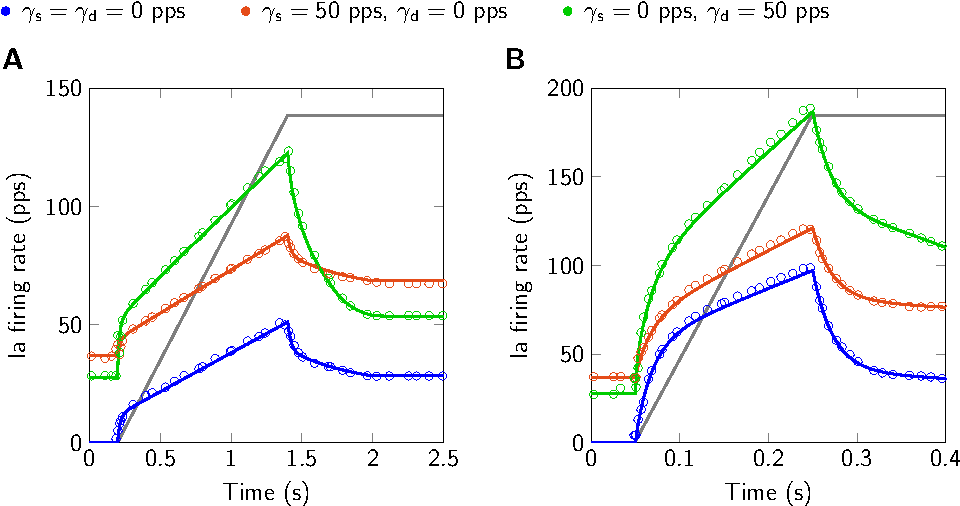
\includegraphics[width=\textwidth]{Figure1.pdf}
    \caption{Model responses (solid lines) to ramp-and-hold stretches and results from \citet{maltenfort2003}, their Fig. 4A and B (circles).  The displacement is qualitatively shown in gray (\SI{6}{\milli\meter} ramp-and-hold stretch). A: ramp velocity \SI{5}{\milli\meter\per\second}. B: ramp velocity \SI{30}{\milli\meter\per\second}. Ia firing rate and static ($\gamma_\mathrm{s}$) and dynamic ($\gamma_\mathrm{d}$) fusimotor drive are given in pulses per second (pps). This figure is created by running Fig01.m.}
    \label{fig:fig4}
\end{figure}

% Figure 2
\begin{figure}
    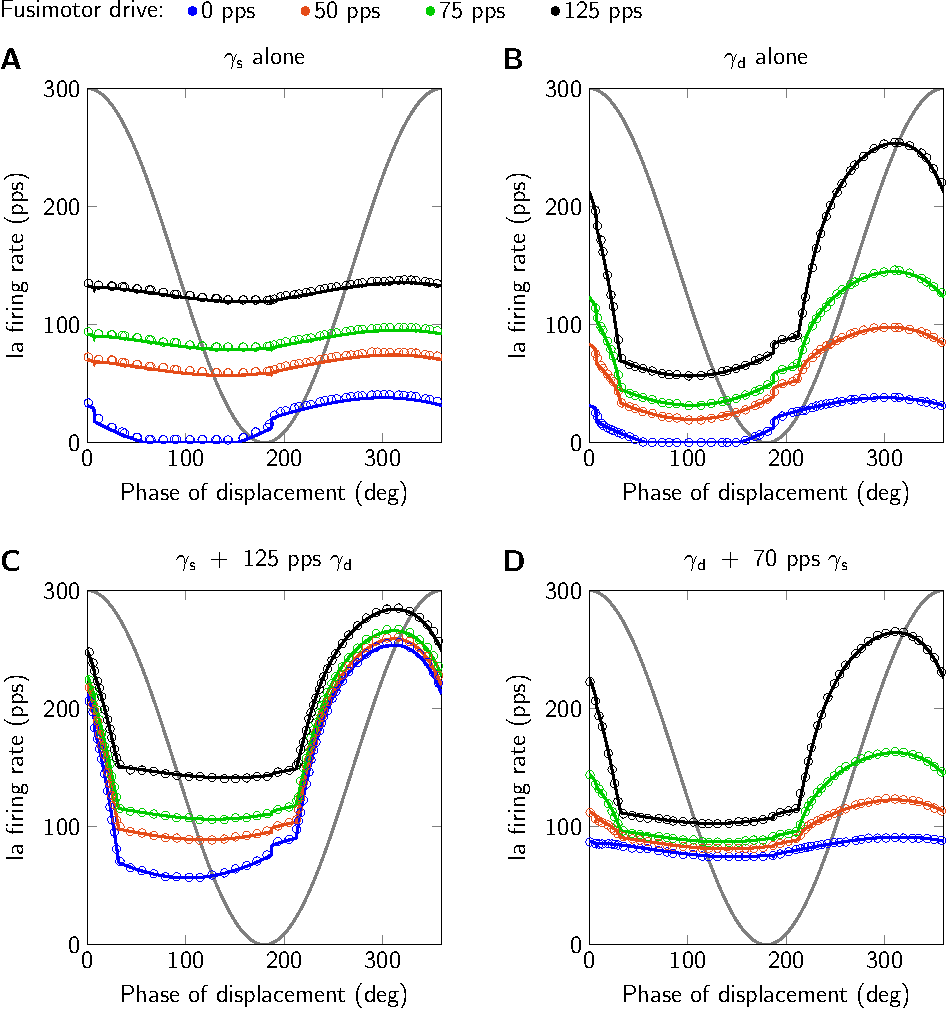
\includegraphics[width=\textwidth]{Figure2.pdf}
    \caption{Model responses (solid lines) to sinusoidal stretch and results from \citet{maltenfort2003}, their Fig. 5 (circles). The displacement is qualitatively shown in gray (\SI{1.4}{\milli\meter} peak-to-peak sinusoidal stretch, mean displacement \SI{4}{\milli\meter}, frequency 1 Hz, second of two cycles). A: only static fusimotor drive ($\gamma_\mathrm{s}$). B: only dynamic fusimotor drive ($\gamma_\mathrm{d}$). C: static fusimotor drive against a tonic background of dynamic fusimotor drive. D: dynamic fusimotor drive against a tonic background of static fusimotor drive. Ia firing rate and fusimotor drive are given in pulses per second (pps). This figure is created by running Fig02.m.}
    \label{fig:fig5}
\end{figure}

% Figure 3
\begin{figure}
    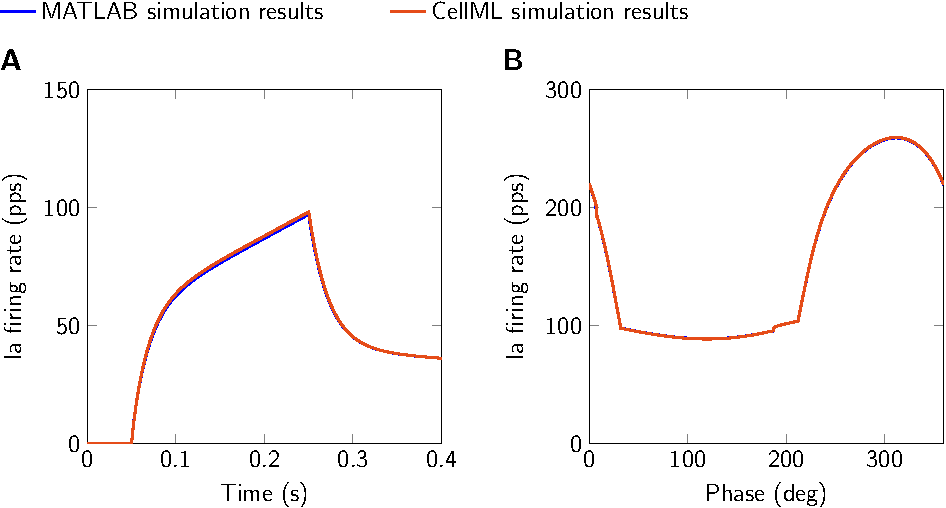
\includegraphics[width=\textwidth]{Figure3.pdf}
    \caption{Comparison of simulation results obtained with MATLAB and CellML implementations. A: \SI{6}{\milli\meter} ramp-and-hold stretch, ramp velocity \SI{30}{\milli\meter\per\second}, no fusimotor drive. B:  Sinusoidal stretch (\SI{1.4}{\milli\meter} peak-to-peak, mean displacement \SI{4}{\milli\meter}, frequency 1 Hz, second of two cycles), static gamma drive 50 pps, dynamic gamma drive 125 pps. Ia firing rate and fusimotor drive are given in pulses per second (pps). This figure is created by running both, Fig03.sedml and Fig03.m.}
    \label{fig:fig3}
\end{figure}


\section{Reproducability goals}\label{sec:reprod}
% Figures showing that the code simulates the same graphs as shown in the  primary paper.
The aim of this paper is to provide a model which is able to reproduce the results as shown in Fig.~4A and Fig.4B as well as Fig.~5A-D of the original publication. 
Since the data from the original publication were not available, Engauge Digitizer (Version 10.4) was used to obtain the data points shown herein.\\
In Fig.~\ref{fig:fig4} spindle responses to ramp-and-hold stretches of two different ramp velocities are shown.
The prediction of the simulations coincide very well with the digitized data from the original publication. 
The same applies for simulation results in response to sinusoidal stretches as shown in Fig.~\ref{fig:fig5}.
Here, the second of two stretch cycles is plotted to exclude effects from the initial displacement at the beginning of the first stretch cycle. 
Note that small deviations from the digitized data have their origin in unavoidable inaccuracies due to figure resolution and choice of line styles. \\
The CellML code was run exemplary for two scenarios to show the consistency with the MATLAB model. 
As it can be seen in Fig.~\ref{fig:fig3}A, the CellML prediction is slightly higher during the ramp phase of the ramp-and-hold scenario. 
This is due to the necessary modification to the implementation of the velocity filter (cf. Section~\ref{sec:modifications}) and the difference is  dependent on the chosen solver and time step size. 
However, the deviations are  small and even less pronounced for the sinusoidal stretch with applied fusimotor drive (cf. Fig.~\ref{fig:fig3}B).

\section{Discussion}
%  Discuss the results, strengths and limitations of the model, and point to future developments and uses. 
With this publication, a corrected version of the \citet{maltenfort2003} muscle spindle model is made available to facilitate the integration of muscle spindle models in future models of the neuromuscular system. 
The overestimation of the spindle firing rate in response to dynamic fusimotor drive, as also addressed by \citet{grandjean2014}, is corrected in the provided model. 
It was shown that the provided codes reproduce the results published in the original paper. 
As shown in \citet{maltenfort2003}, these results match a variety of experimentally observed characteristics of muscle spindle firing. 
For an elaborate discussion of the model, the reader is referred to the original publication \citep{maltenfort2003}. \\
In absence of secondary afferent firing, the model is well suited for large-scale bio-physically motivated simulations due to its low computational cost (cf. e.\,g. \citealp{rohrle2019}). 
% Further, combining the spindle model with a continuum-mechanical muscle model (e.\,g. \citet{heidlauf2017}) has the potential to provide new means of investigating muscle spindle behaviour.
%Further, musculo-skeletal models involving multiple muscles (e.g. the currently purely continuum-mechanical model of \citet{roehrle2017}) can be extended by integrating a muscle spindle model to investigate sensory interactions across joints. 
For example, combining the spindle model with a continuum-mechanical multi-muscle model (e.\,g. \citealp{roehrle2017}) has the potential to provide new means of investigating muscle spindle behaviour in response to heterogeneous muscle deformations as well as sensory interactions across joints.


\FloatBarrier

\section*{Acknowledgements}
This research was funded by the Deutsche Forschungsgemeinschaft (DFG, German Research Foundation) under Germany’s Excellence Strategy EXC 2075 (390740016) and SPP 2311 (RO 4019/7-1).

\bibliography{MB03}

\end{document}